\documentclass[aspectratio=169]{beamer}

\setbeamersize{text margin left=5mm, text margin right=5mm}

\defbeamertemplate{headline}{my header}{%
\vskip1pt%
\makebox[0pt][l]{\,\insertshortauthor}%
\hspace*{\fill}\insertshorttitle/\insertshortsubtitle\hspace*{\fill}%
\llap{\insertpagenumber/\insertpresentationendpage\,}
}
\setbeamertemplate{headline}[my header]

\let\olditem\item
\renewcommand{\item}{\setlength{\itemsep}{\fill}\olditem}

\usepackage{caption}
\usepackage{soul}
\usepackage{tkz-euclide}
\usetikzlibrary{calc}
\usepackage[]{algorithm2e}
\usepackage{changepage}
\usepackage{amssymb}
\usepackage{bm}
\usepackage{xcolor}
\usepackage{mathtools}
\usepackage{tcolorbox}
\usepackage{tikz}
\usepackage{tikz-3dplot}
\usetikzlibrary{arrows.meta, decorations.pathreplacing, positioning, shapes.geometric}
\usepackage{extarrows}


%% Fonts
\usefonttheme{professionalfonts}
\usefonttheme{serif}

\DeclareCaptionLabelFormat{blank}{}
\captionsetup[figure]{labelformat=blank}

%% Math definitions
\def\mf{\ensuremath\mathbf}
\def\mb{\ensuremath\mathbb}
\def\mc{\ensuremath\mathcal}
\def\lp{\ensuremath\left(}
\def\rp{\ensuremath\right)}
\def\lv{\ensuremath\left\lvert}
\def\rv{\ensuremath\right\rvert}
\def\lV{\ensuremath\left\lVert}
\def\rV{\ensuremath\right\rVert}
\def\lc{\ensuremath\left\{}
\def\rc{\ensuremath\right\}}
\def\ls{\ensuremath\left[}
\def\rs{\ensuremath\right]}
\def\bmx{\ensuremath\begin{bmatrix*}[r]}
\def\emx{\ensuremath\end{bmatrix*}}
\def\bmxc{\ensuremath\begin{bmatrix*}[c]}
\def\t{\lp t\rp}
\def\k{\ls k\rs}

\newcommand{\demoex}[2]{\onslide<#1->\begin{color}{black!60} #2 \end{color}}
\newcommand{\demoexc}[3]{\onslide<#1->\begin{color}{#2} #3 \end{color}}
\newcommand{\anim}[3]{\onslide<#1->{\begin{color}{#2!60} #3 \end{color}}}
\newcommand{\ct}[1]{\lp #1\rp}
\newcommand{\dt}[1]{\ls #1\rs}
\newcommand{\cols}[2]{\begin{columns}[#1] #2 \end{columns}}
\newcommand{\col}[2]{\begin{column}{#1} #2 \end{column}}

%% Mycolors
\definecolor{myred}{RGB}{192,0,0}
\definecolor{mygray}{RGB}{100,100,100}

%% Custom beamer color
\setbeamercolor{title}{fg=myred}
\setbeamercolor{subtitle}{fg=myred}
\setbeamerfont{title}{series=\bfseries}
% \setbeamercolor{frametitle}{bg=myred, fg=white}
\setbeamercolor{frametitle}{bg=mygray!10!, fg=myred}
\setbeamerfont{frametitle}{series=\bfseries}
\setbeamercolor{item}{fg=mygray}
\setbeamercolor{title in head/foot}{fg=myred}

% Move header to footer
\setbeamertemplate{headline}{}
\setbeamertemplate{footline}{
  \begin{beamercolorbox}[wd=\paperwidth,ht=2.25ex,dp=1ex,center]{footline}
    \inserttitle\hfill\insertauthor\hfill\insertdate\hfill\insertframenumber{}
  \end{beamercolorbox}
}

\title{Applied Linear Algebra in Data Analysis}

% A subtitle is optional and this may be deleted
\subtitle{What is this course about?}

\author{Sivakumar Balasubramanian}
% - Give the names in the same order as the appear in the paper.
% - Use the \inst{?} command only if the authors have different
%   affiliation.

\institute[Christian Medical College] % (optional, but mostly needed)
{
  \inst{}%
  Department of Bioengineering\\
  Christian Medical College, Bagayam\\
  Vellore 632002
}
% - Use the \inst command only if there are several affiliations.
% - Keep it simple, no one is interested in your street address.

\date{}
% - Either use conference name or its abbreviation.
% - Not really informative to the audience, more for people (including
%   yourself) who are reading the slides online

\subject{Lecture notes on ALADA}
% This is only inserted into the PDF information catalog. Can be left
% out. 

% If you have a file called "university-logo-filename.xxx", where xxx
% is a graphic format that can be processed by latex or pdflatex,
% resp., then you can add a logo as follows:

% \pgfdeclareimage[height=0.5cm]{university-logo}{university-logo-filename}
% \logo{\pgfuseimage{university-logo}}

% Delete this, if you do not want the table of contents to pop up at
% the beginning of each subsection:
\AtBeginSubsection[]
{
  \begin{frame}<beamer>{Outline}
    \tableofcontents[currentsection,currentsubsection]
  \end{frame}
}

% Let's get started
\begin{document}

\begin{frame}
  \titlepage
\end{frame}


\begin{frame}[t]{What is this course about?}
  \vspace{2cm}
  \begin{center}
    \textcolor{myred}{\huge \textbf{This is an introductory course of high dimensional thinking.}}
  \end{center}
\end{frame}


\begin{frame}[t]{The world is multidimensional}
\begin{itemize}
  \item Most things/systems/ideas of interest in science and engineering are multidimensional.
  \item Most courses in undergraduate engineering programs focus on mathematical skills for representing, analysing, and designing simple systems $\longrightarrow$ Univariate \textbf{Calculus}!
  \begin{itemize}
    \item Linear single-input-single-output (SISO) system theory (used in signal processing and control theory).
    \item Fourier, Laplace, z-transforms for understanding 1D temporal or spatial phenomena.
    \item Study of dynamics in mechanical engineering.
  \end{itemize}
  \item Most applications or systems we deal with have multiple degree-of-freedom, various causes and effects, multiple inputs and outputs, multiple measurements, multiple parameters etc.
  \item Dealing with such multidimensional problems requires an additional set of mathematical tools and a different way of thinking. 
\end{itemize}
\end{frame}


\begin{frame}{What are these multidimensional problems?}
  \begin{columns}
    \begin{column}{0.3\textwidth}
      \begin{itemize}
        \item Signal processing
        \item Control theory
        \item Robotics
        \item Statistics
        \item Machine learning
        \item Optimization
        \item $\cdots$
      \end{itemize}
    \end{column}
    \begin{column}{0.675\textwidth}
      \begin{figure}
        \centering
        
\includegraphics[width=0.8\textwidth]{toomany.png}
      \end{figure}
    \end{column}    
  \end{columns}
\end{frame}


\begin{frame}{Signal Processing}
  We often deal with temporal signal that can be visualized as a function of time. Is this the only way to represent a signal?
  \vspace{0.2cm}

  A sinusoidal signal's time domain representation is shown below. We don't need the signal's entire time record to covney its information. We only need three numbers - the amplitude, frequency, and phase of the sinusoid. These are sufficient to reconstruct the signal. They can be obtained by Fourier transforming the signal into the frequency domain, i.e. a different perspective of the signal.
  \begin{figure}
    \centering
    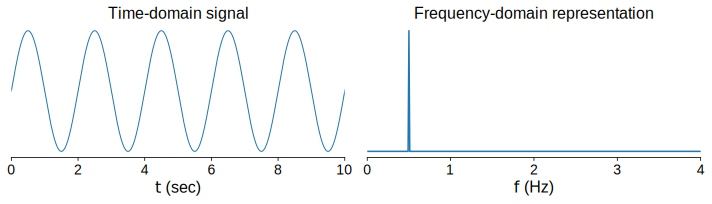
\includegraphics[width=0.8\textwidth]{../../analysis/signalprocessing/output/signal1_fft.png}
  \end{figure}
\end{frame}


\begin{frame}{Signal Processing}
  We can do this to slightly more complex signals as well:
  \vspace{0.2cm}

  \begin{figure}
    \centering
    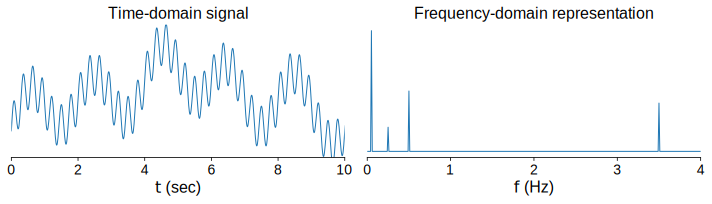
\includegraphics[width=0.8\textwidth]{../../analysis/signalprocessing/output/signal2_fft.png}
  \end{figure}

  \textcolor{red}{What is so special about the Fourier transform? Are there other transforms that might better suited for certain types of signals? Can I design my own transform?}
  \vspace{0.2cm}

  Thinking of signals and images as entities residing in a high-dimensional space turns out to be very useful way to think about signals and how to process them.
\end{frame}


\begin{frame}{Control theory}
  \begin{columns}
    \begin{column}{0.5\textwidth}
      \vspace{0.2cm}
      A spacecraft has 6 DOF - 3 translational $x, y, z$ and 3 rotational $\phi_1, \phi_2, \phi_3$.

      We need both position and velocity information to control the spacecraft.
      \vspace{0.2cm}
      
      The spacecraft has multiple sensors that measure position and velocity.
      \vspace{0.2cm}
      
      Multiple thrusters, reaction-wheels are used to control the spacecraft dynamics.
      \vspace{0.2cm}

      \textcolor{red}{How do we get the best estimate of the spacecraft position and velocity? Which and by how much do we activate the different thrusters and reaction-wheels to control the spacecraft?}
    \end{column}
    \begin{column}{0.475\textwidth}
      \begin{figure}
        \centering
        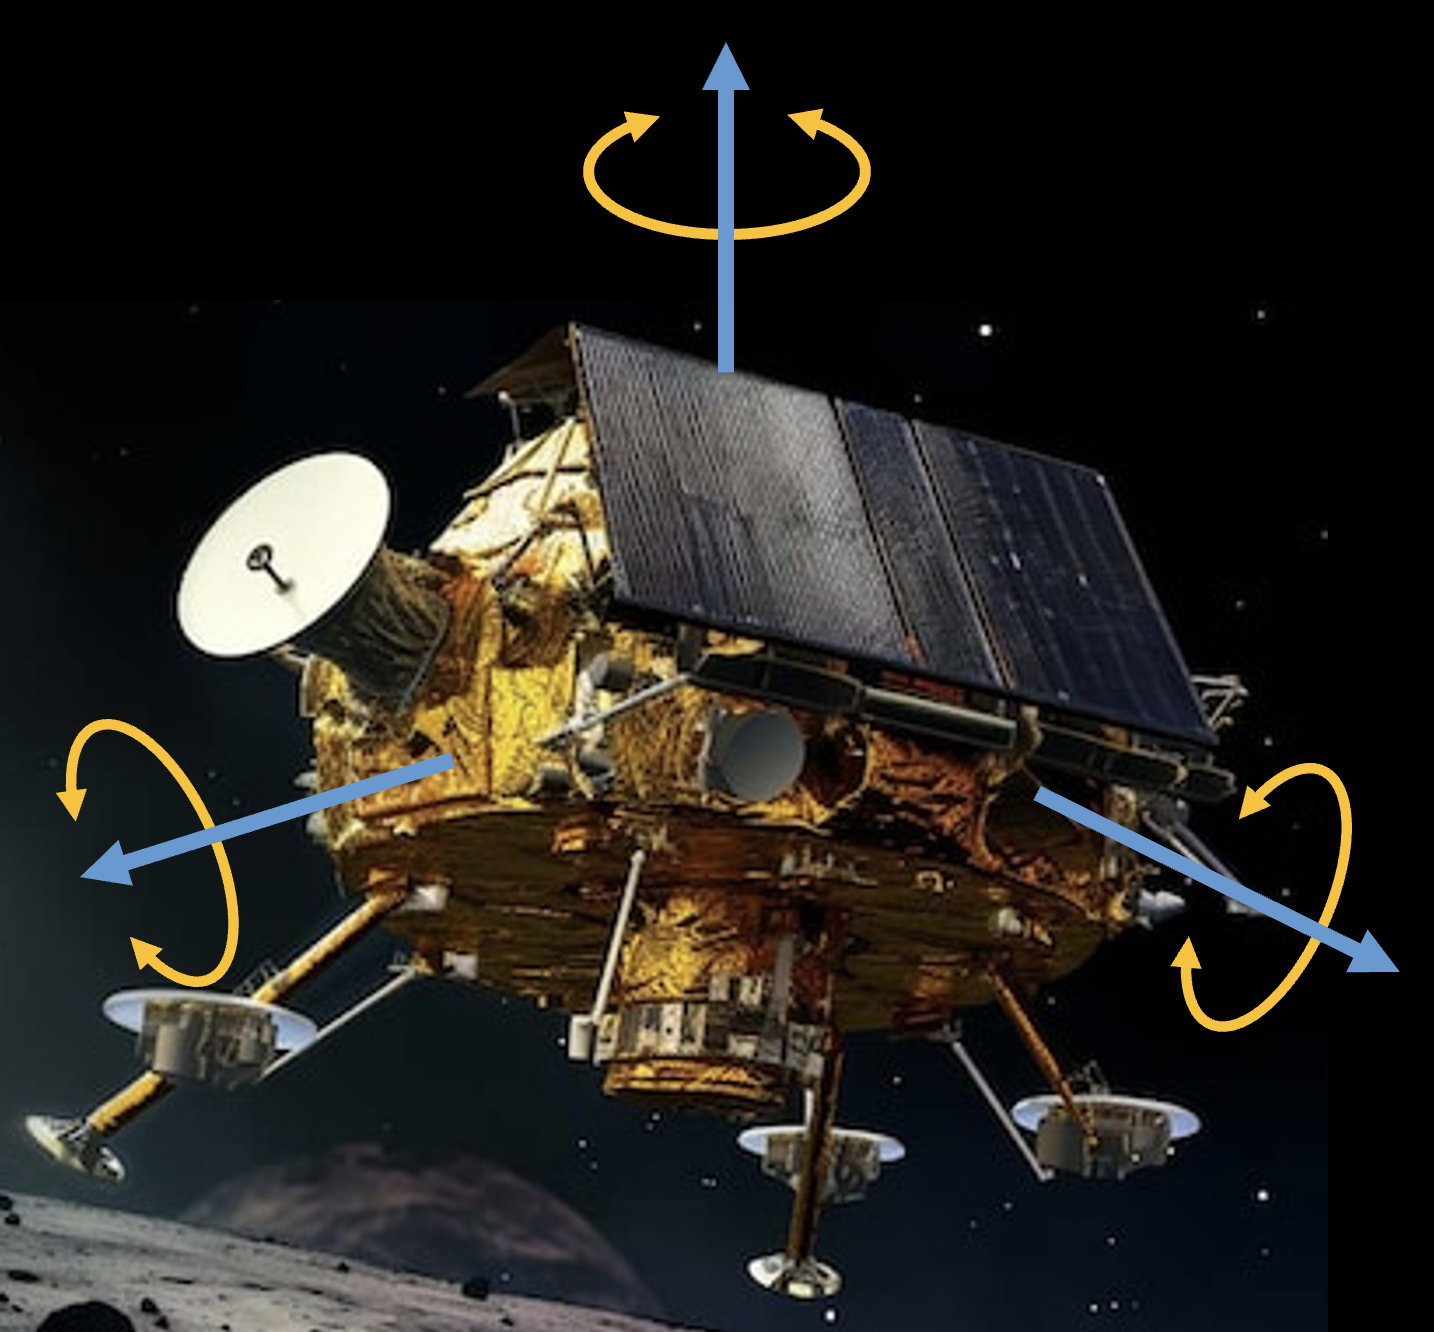
\includegraphics[width=1\textwidth]{spacecraft.png}
        \caption{\scriptsize Source: http://surl.li/klulx}
      \end{figure}
    \end{column}    
  \end{columns}
\end{frame}


\begin{frame}{Robotics}
  \begin{columns}
    \begin{column}{0.475\textwidth}
      \begin{figure}
        \centering
        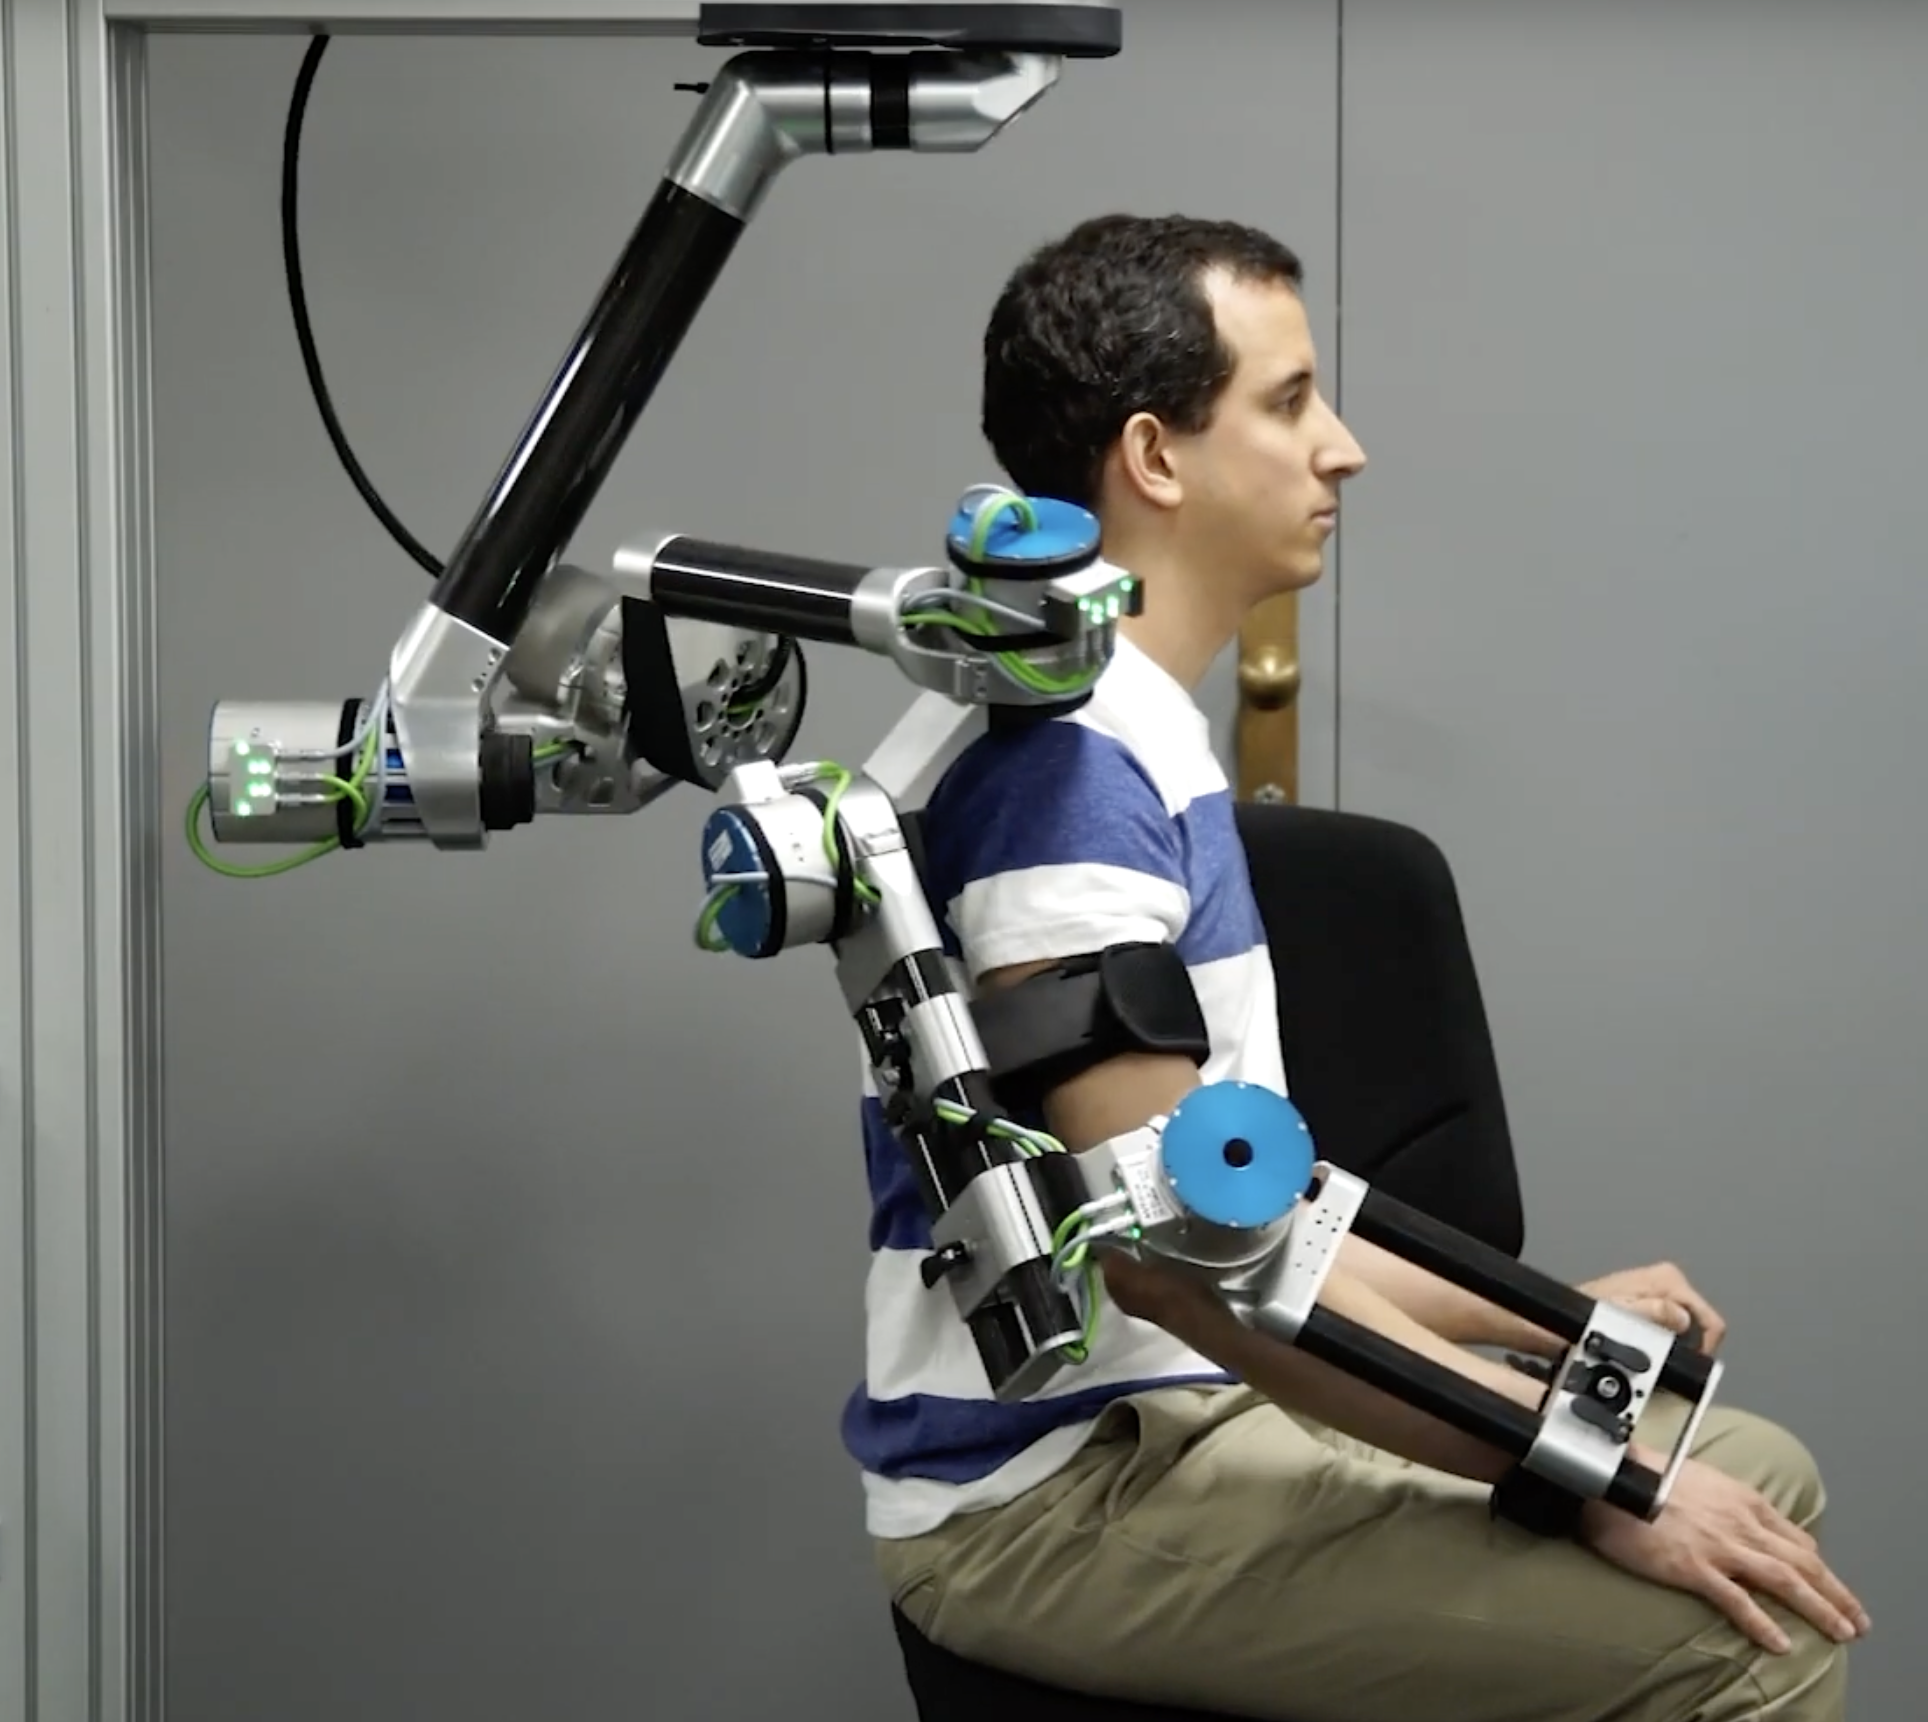
\includegraphics[width=0.825\textwidth]{rehabrobots.png}
        \caption{\scriptsize \textbf{Rehab Robot} [Source: http://surl.li/klupd]}
        % 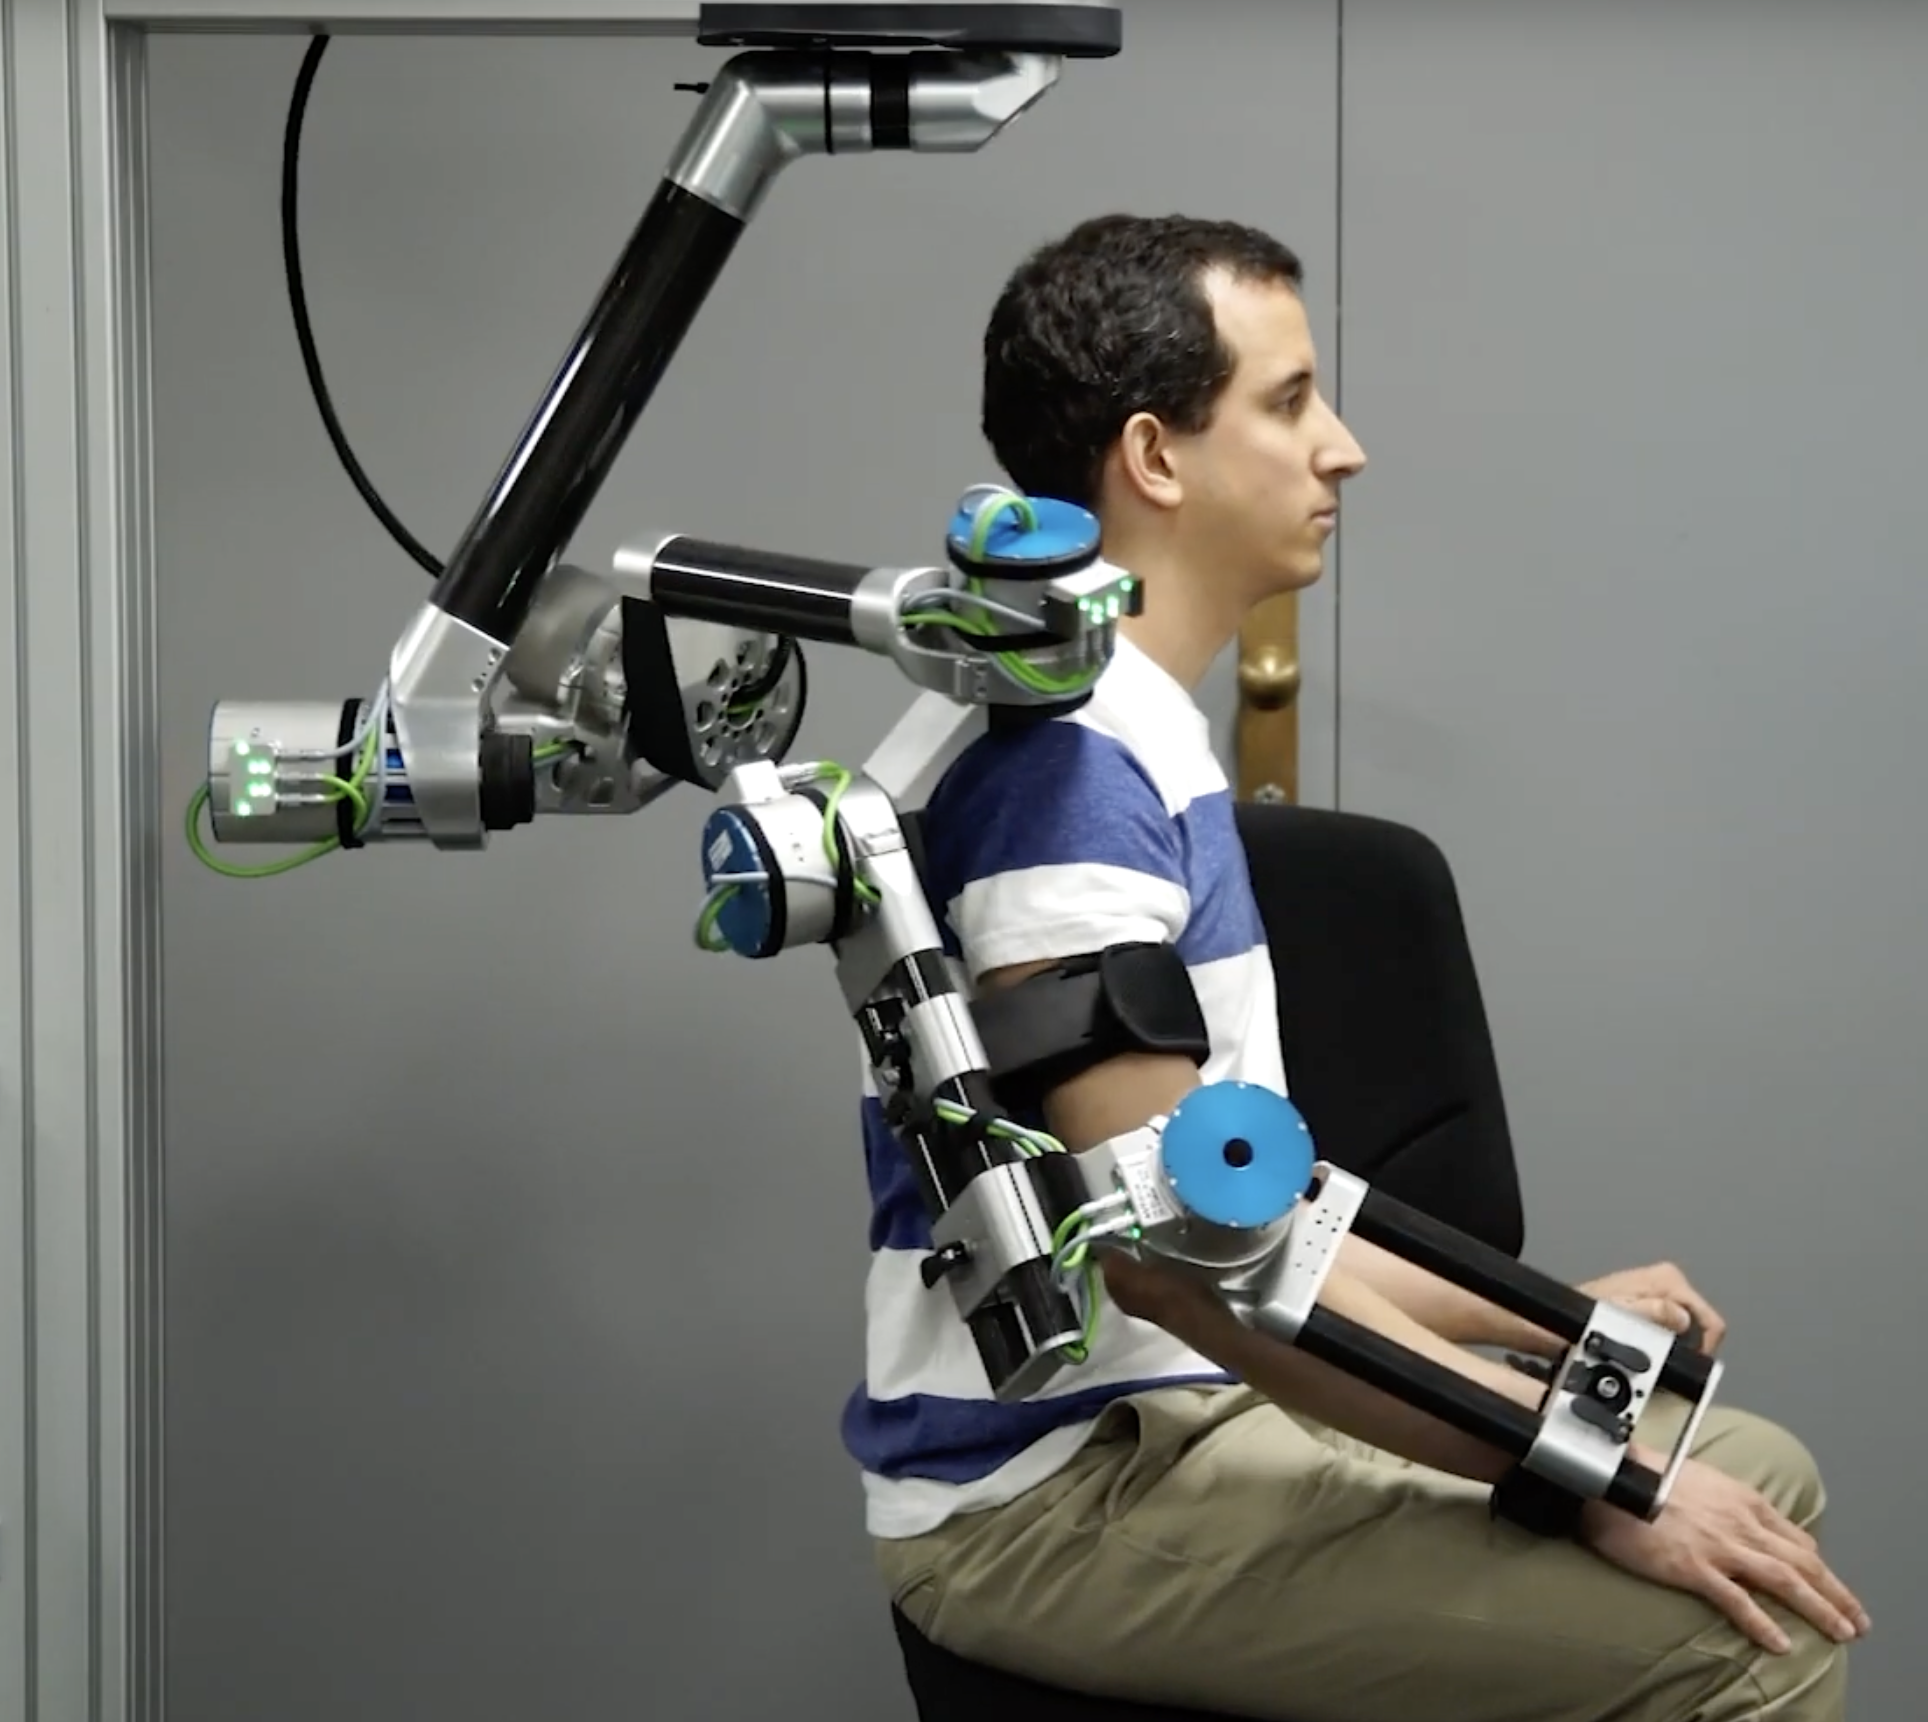
\includegraphics[width=1\textwidth]{rehabrobots.png}
        % \caption{\scriptsize Source: http://surl.li/klurm}
      \end{figure}
    \end{column}
    \begin{column}{0.5\textwidth}
      \begin{figure}
        \centering
        % 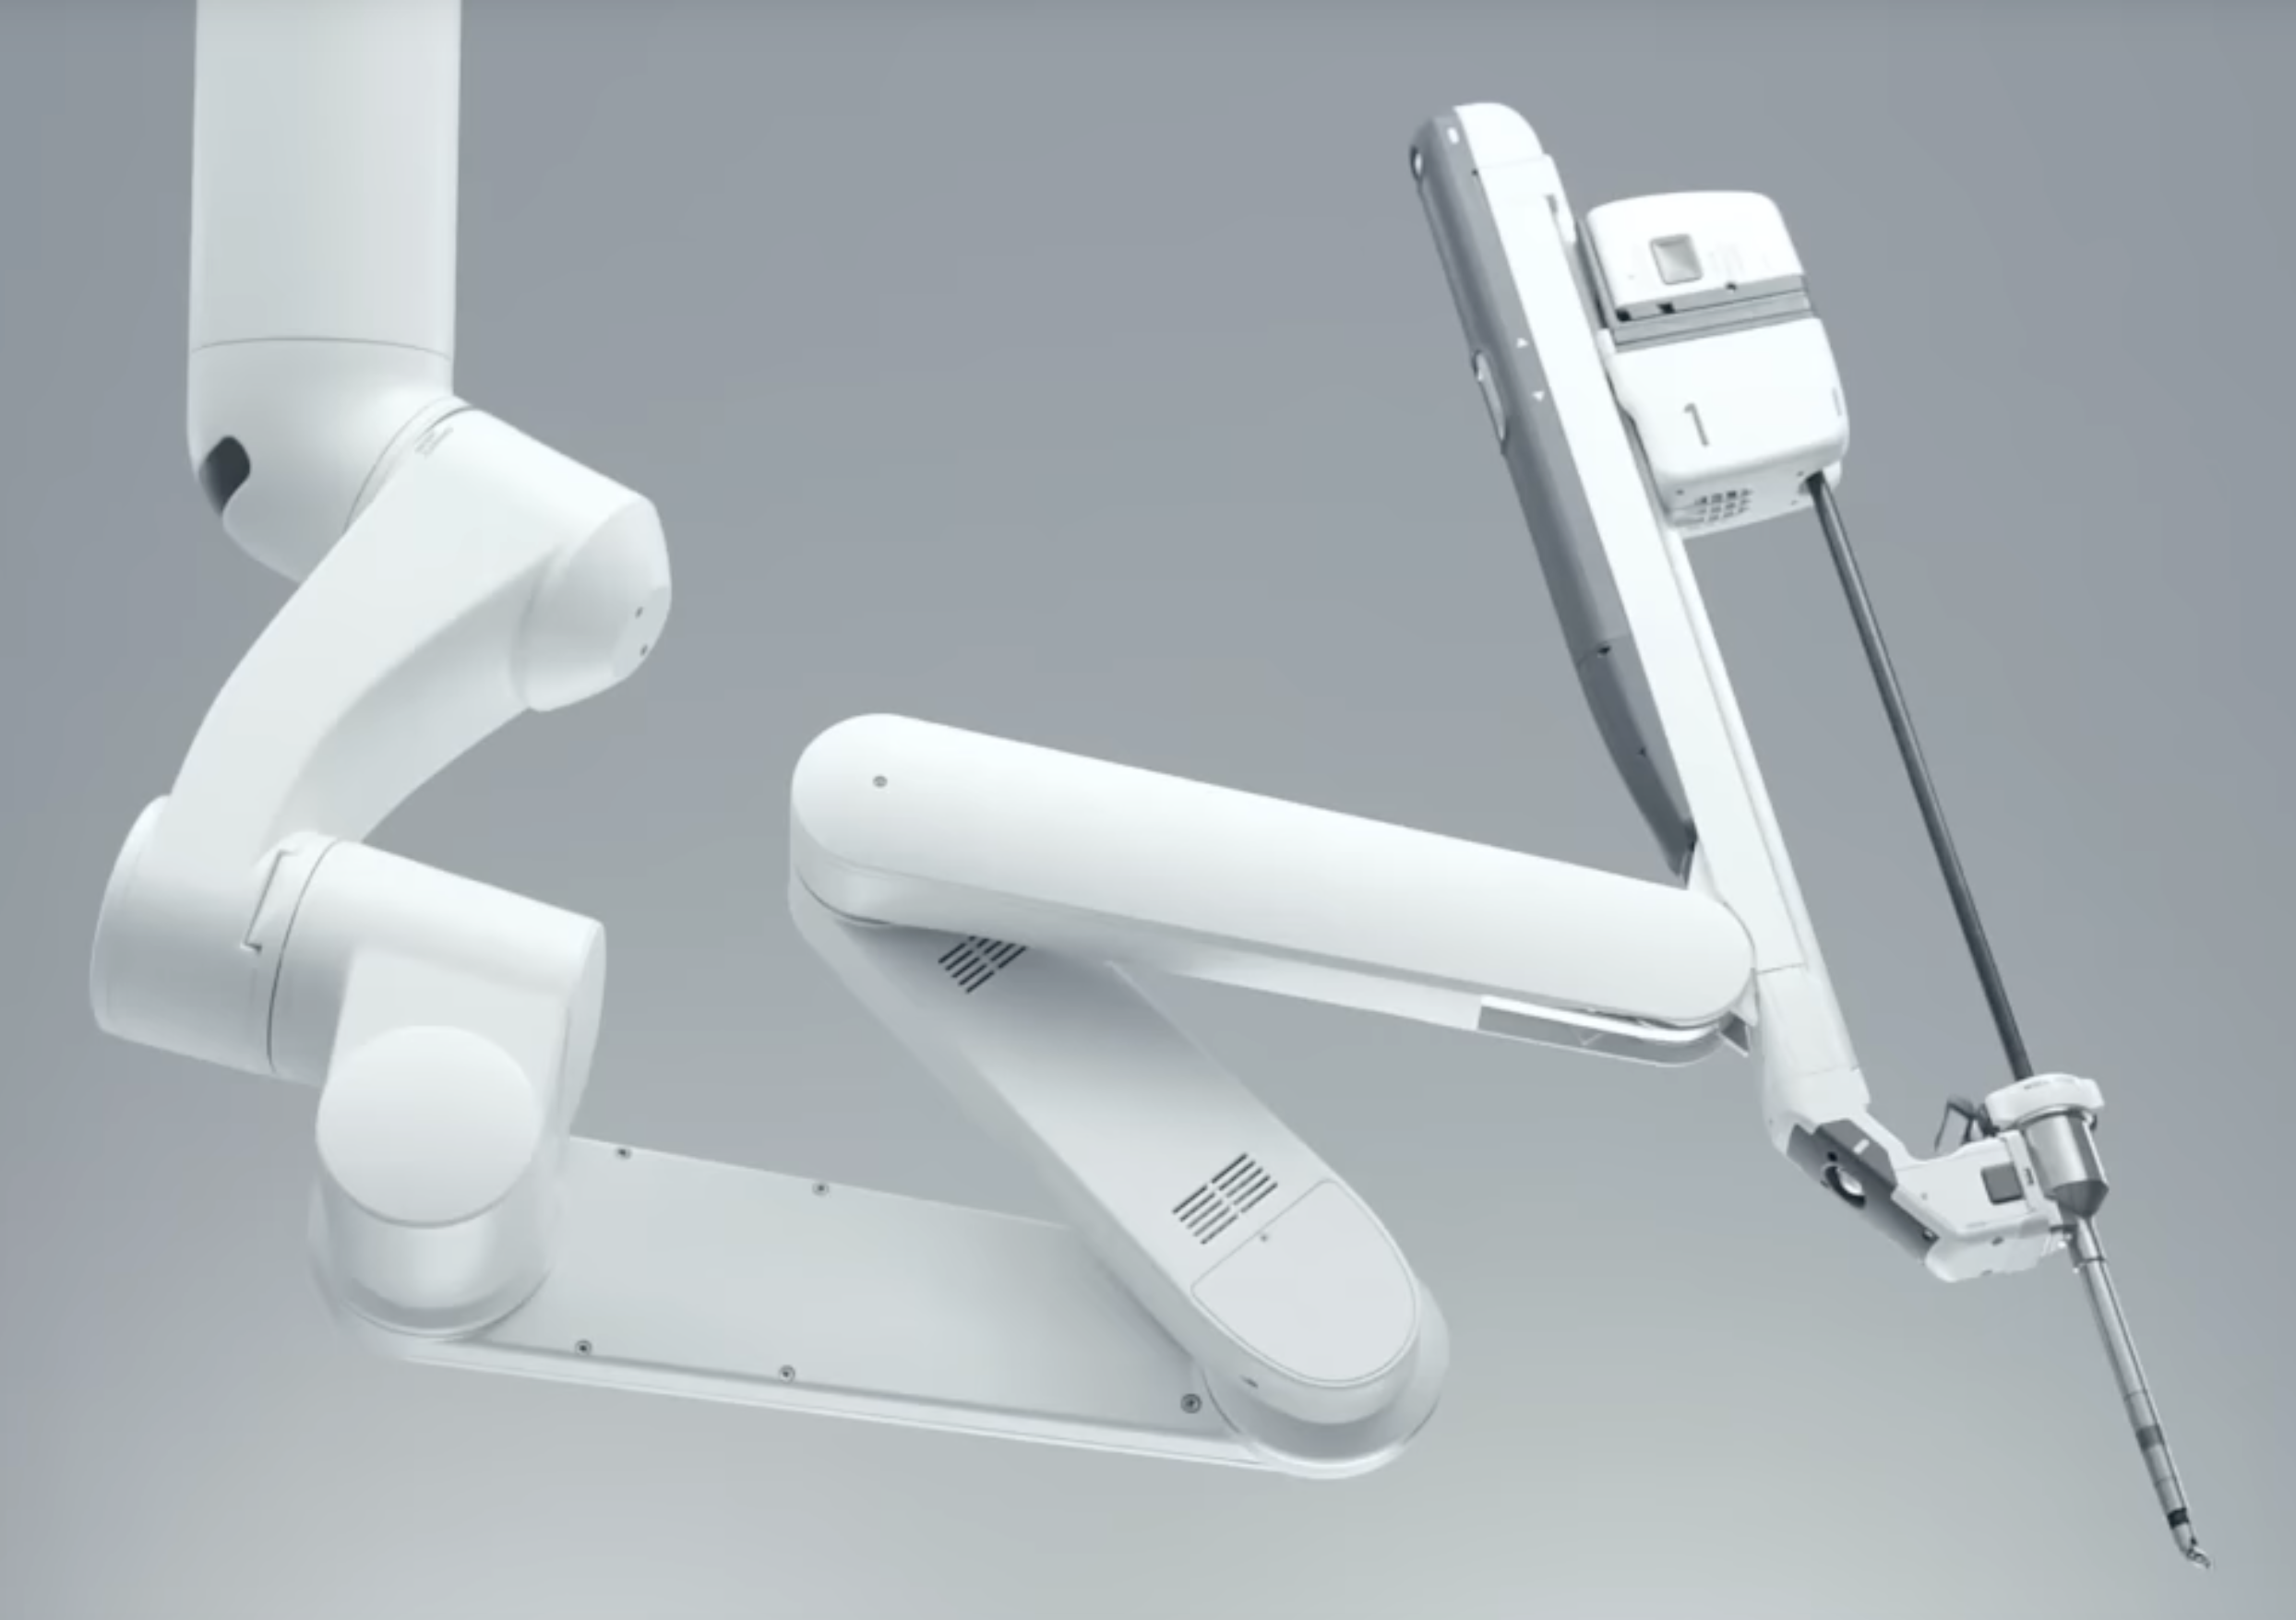
\includegraphics[width=1\textwidth]{surgicalrobot.png}
        % \caption{\scriptsize Source: http://surl.li/klupd}
        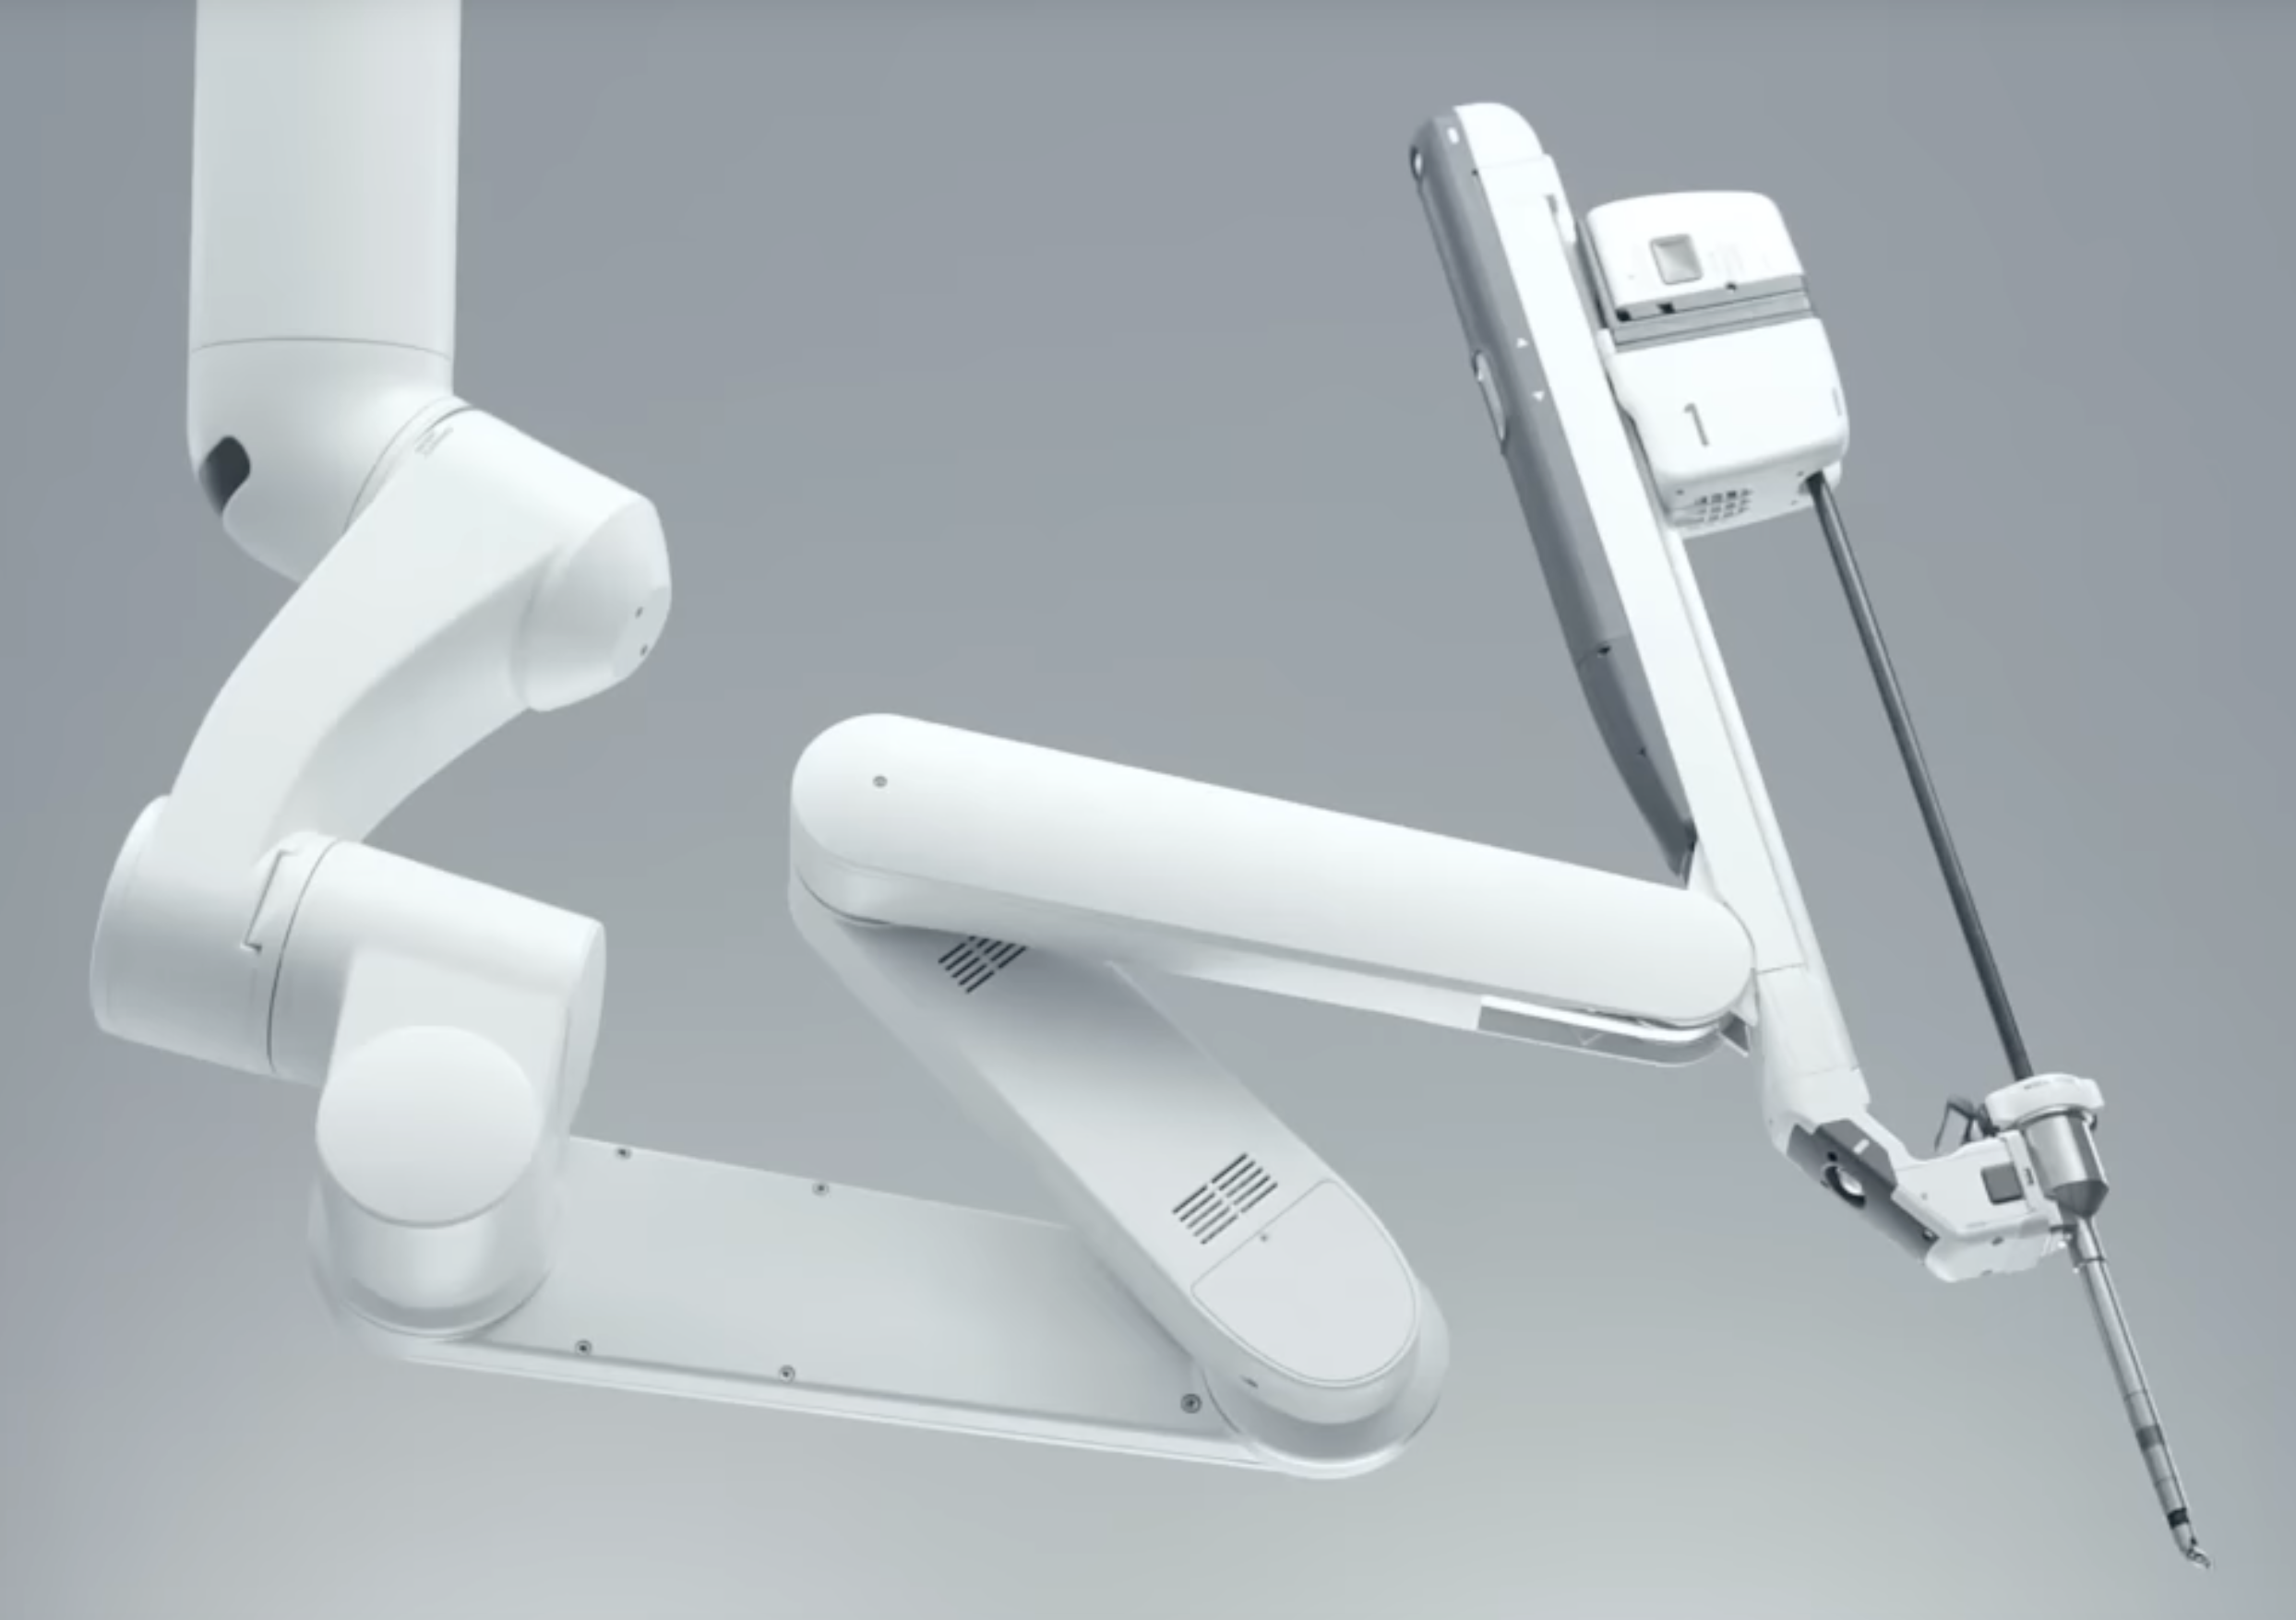
\includegraphics[width=1\textwidth]{surgicalrobot.png}
        \caption{\scriptsize \textbf{Surgical Robot} [Source: http://surl.li/klurm]}
      \end{figure}
    \end{column}    
  \end{columns}
\end{frame}


\begin{frame}{Robotics}
  Typically robots have multiple DOF.
  \vspace{0.2cm}
  
  The end-effector of the robot is often where interesting things happen. 
  \vspace{0.2cm}
  
  Controlling the kinematics of the end-effector and its interaction with evnironment (forces and torques) through multiple actuators and sensors located on the robot's body poses a multidimensional control problem.
  \vspace{0.2cm}

  \textcolor{red}{Which and by how much do we activate the different actuators to control the end-effector?}
\end{frame}


\begin{frame}{Statistics}
  The data that we deal with is often heterogeneous, high-dimensional, and noisy.
  \vspace{0.2cm}
  
  Representing such data, evaluating the relationships between different variables, building models for inference and estimation of natural phenomena is at the core of statistics. 
  \vspace{0.2cm}
  
  There is a need for mathematical frameworks and computaitonal methods for doing these efficiently.
  \vspace{0.2cm}
  
  \textbf{Example}: How much do dietry habits, alchohol consumption, smoking, exercise, and other lifestyle factors affect the risk of developing a stroke? We want to identify the most important factor and strength of its effect.

  \textcolor{red}{How do we do answer this question, assuming we have data collected from a large segments of the population over several years?}
\end{frame}


\begin{frame}{Machine learning}
  In machine learning, we are interested in predicting, and automating complex relationships and tasks through the use of data.
  \vspace{0.2cm}
  
  Data is almost always high dimensional in such applications with complex structure.
  \vspace{0.2cm}
  
\end{frame}


\begin{frame}[t]{Linear Algebra - the workhorse of modern science and engineering}
\begin{figure}
  \centering 
  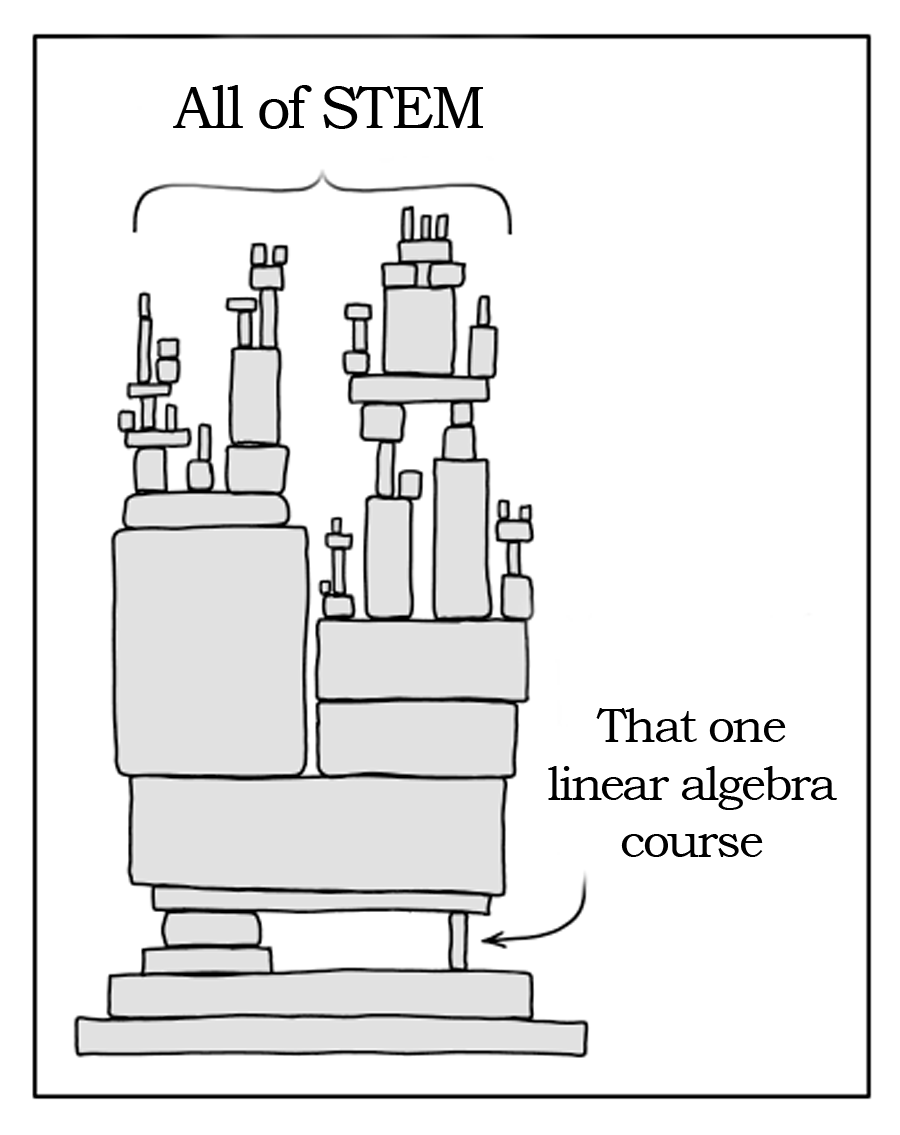
\includegraphics[width=0.35\textwidth]{../../truth.png}
\end{figure}
\end{frame}


\begin{frame}[t]{Linear Algebra}
\begin{itemize}
  \item Algebra (Arabic: \textit{al-jabr} `reunion of broken parts') is the study of variables and the rules for manipulating these variables in formulas (Source: Wikipedia).
  
  \item Linear algebra is the study of linear system of equations.
  \[
    \begin{split}
      a_{11} x_1 + a_{12} x_2 + a_{13} x_3 &+ \cdots + a_{1n} x_n = y_1\\
      &\vdots \\ 
      a_{m1} x_1 + a_{32} x_2 + a_{m3} x_3 &+ \cdots + a_{mn} x_n = y_m
    \end{split}
  \]
  These are useful in a surprisingly wide range of real world problems!
  \[ 
    \begin{split}
      x_1, x_2, \ldots x_n &: \text{inputs/parameters of the problem}\\
      y_1, y_2 \ldots y_m &: \text{outputs or mesaurements}\\
      a_{ij} &: \text{physics of the problem}
    \end{split}
  \]
  \item Linear algebra provides tools for: understanding, manipulating, and efficiently solving such problems.
\end{itemize}
\end{frame}


\begin{frame}{Linear algebra in engineering: Signal Processing}
  \begin{itemize}
    \item Expressing signals as a linear combinations of other signals (basis functions) is at the core of most of signal processing.
    \[ x\ct{t} = c_1 \phi_1\ct{t} + c_2 \phi_2\ct{t} + \cdots + c_n \phi_n\ct{t} \]

    \item $\lc c_i \rc_{i}$ is another representation of the signal $x\ct{t}$ in terms of $\lc \phi_i\ct{t} \rc_i$.
    
    \item $\lc \phi_i \rc_{i}$ are called the basis functions.  Different basis functions gives different types of transforms.
    
    \item Manipulating $\lc c_i \rc_i$ will allow us to extract or suppress different types of information from $x\ct{t}$.
  \end{itemize}
\end{frame}


\begin{frame}{Linear algebra in engineering: Signal Processing}
  \begin{figure}
    \centering
    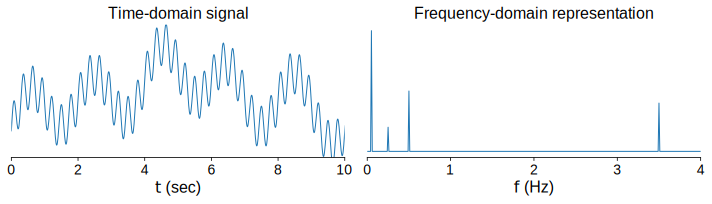
\includegraphics[width=0.8\textwidth]{../../analysis/signalprocessing/output/signal2_fft.png}
  \end{figure}
\end{frame}


\begin{frame}{Linear algebra in engineering: Robotics}
  \begin{columns}
    \begin{column}{0.5\textwidth}
      Kinematics and dynamics of serial robots are highly non-linear.

      \textbf{Kinematics of a 2-link planar robot}
      \[ 
        \begin{split}
          x &= l_1 \cos\ct{\theta_1} + l_1 \cos\ct{\theta_1 + \theta_2} \\
          y &= l_1 \sin\ct{\theta_1} + l_1 \sin\ct{\theta_1 + \theta_2} \\
        \end{split}
      \]

      The differential kinematics however has is linear relationship:
      \[ \bmx \dot{x} \\ \dot{y}\emx = \mf{J}\ct{\theta_1, \theta_2} \bmx \dot{\theta}_1 \\ \dot{\theta}_2 \emx \]
      \[ \mf{J}\ct{\theta_1, \theta_2}: \text{Jacobian matrix} \]
    \end{column}
    \begin{column}{0.45\textwidth}
      \begin{figure}
        \centering
        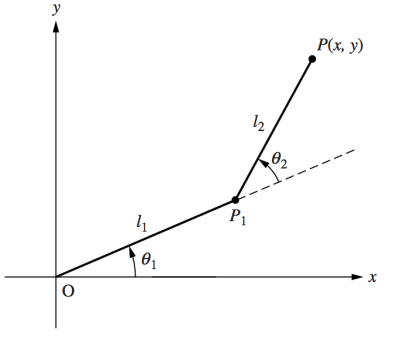
\includegraphics[width=0.8\textwidth]{2links.png}
      \end{figure}
    \end{column}    
  \end{columns}
\end{frame}


\begin{frame}{Linear algebra in engineering: Robotics}
  \begin{columns}
    \begin{column}{0.5\textwidth}
      \textbf{Dynamics of serial robots.}
      \[ 
        \mf{M}\ct{\mf{q}} \ddot{\mf{q}} + \mf{C}\ct{\mf{q}, \dot{\mf{q}}} \dot{\mf{q}} + \mf{g}\ct{\mf{q}} = \bm{\tau} + \mf{J}^\top \mf{f}
      \]
      where,
      \begin{itemize}
        \item $\mf{q}$: Joint angles
        \item $\mf{M}\ct{\mf{q}}$: Inertia matrix
        \item $\mf{C}\ct{\mf{q}, \dot{\mf{q}}}$: Coriolis and centrifugal forces
        \item $\mf{g}\ct{\mf{q}}$: Gravity forces
        \item $\bm{\tau}$: Joint torques
      \end{itemize}
      
    \end{column}
    \begin{column}{0.45\textwidth}
      \begin{figure}
        \centering
        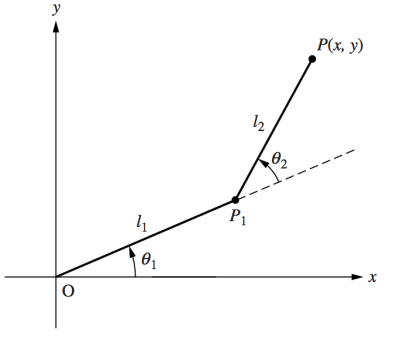
\includegraphics[width=0.8\textwidth]{2links.png}
      \end{figure}
    \end{column}    
  \end{columns}
\end{frame}


\begin{frame}{Linear algebra in engineering: Computed tomography}
  \begin{columns}
    \begin{column}{0.5\textwidth}
      An imagining technique used to obtained detailed images of the inside of an object.
      \vspace{0.2cm}

      A series of images are measurements are taken from different angles around the object. 
      \vspace{0.2cm}

      The measurements are then combined using a mathematical process called \textbf{tomographic reconstruction} to create cross-sectional images of the object.
    \end{column}
    \begin{column}{0.45\textwidth}
      \begin{figure}
        \centering
        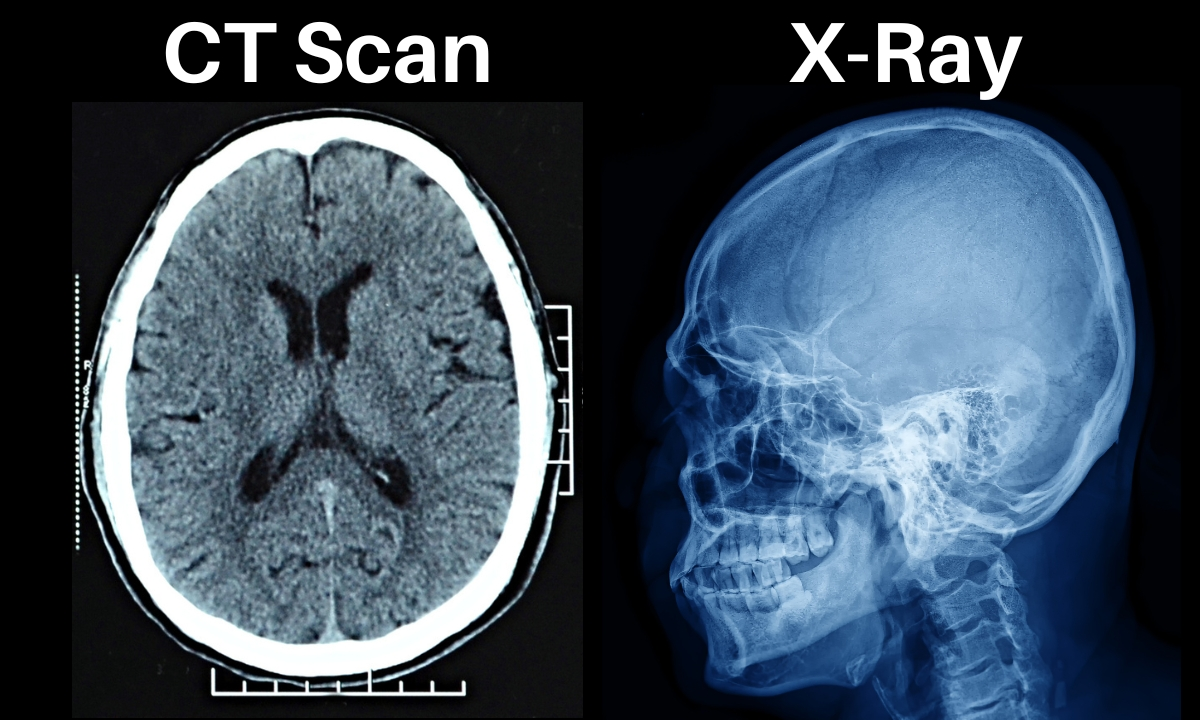
\includegraphics[width=\textwidth]{ctimage.jpg}
      \end{figure}
    \end{column}    
  \end{columns}
\end{frame}


\begin{frame}{Linear algebra in engineering: Computed tomography}
  \begin{figure}
    \centering
    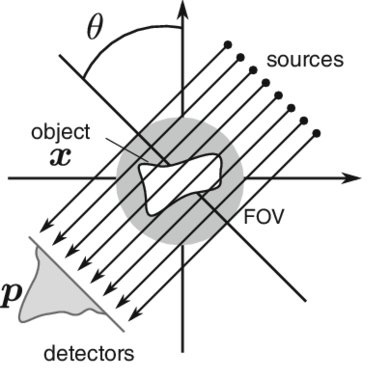
\includegraphics[width=0.45\textwidth]{ct_example.jpg}
  \end{figure}
\end{frame}


\begin{frame}{Linear algebra in engineering}
  \textbf{Machine learning}
  
\end{frame}


\begin{frame}{Linear Algebra - the workhorse of modern science and engineering}

  In a more modern view, linear algebra is the study of vector spaces and linear transformations between them.
\end{frame}



\end{document}